\subsection{Entities, Entity Types, Entity Sets, Attributes}

\begin{figure}[H]
    \centering
    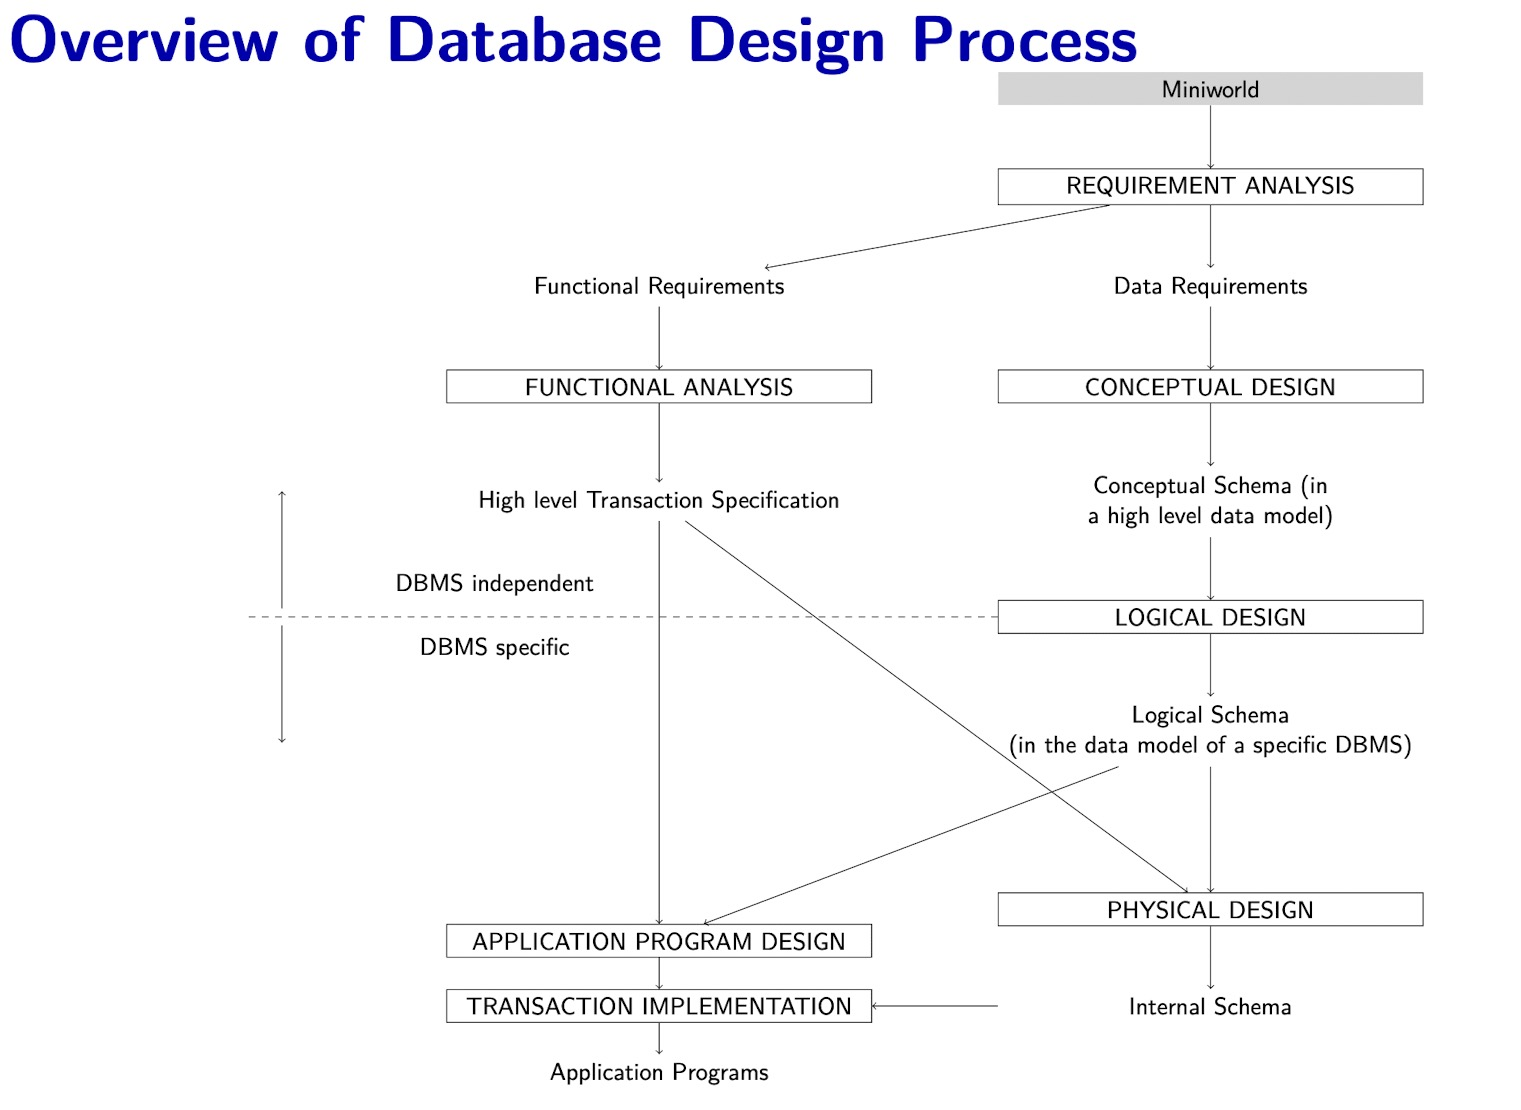
\includegraphics[width=0.75\linewidth]{images/Screenshot 2024-05-22 at 09.59.20.jpg}
\end{figure}


\subsubsection{Entities} 
\begin{itemize}[label=\(\rhd\)]
    \item \textbf{Entities} are specific objects or things in the mini-world that are represented in the database 
    \begin{itemize}[label=\(\rhd\)]
        \item Entity Types:
        \begin{itemize}[label=\(\rhd\)]
            \item Entities with the same basic attributes are grouped or typed into an \textbf{entity type}
            \item An attribute of an entity type for which each entity must have a unique value is called a \textbf{key attribute} of the entity type $\Rightarrow$ each key is \underline{underlined} 
        \end{itemize}
    \end{itemize}
    \item \textbf{Attributes} are properties used to describe an entity
    \begin{itemize}[label=\(\rhd\)]
        \item Attribute Types:
        \begin{itemize}[label=\(\rhd\)]
            \item \textbf{Simple attribute}: each entity has a single atomic value for the attribute
            \item \textbf{Composite attribute}: the attr. may be composed of several components
            \item \textbf{Multi-valued attribute}: an entity may have multiple values for that attribute
            \item \textbf{Derived attribute}: attr. can be derived (computed) rather than stored
        \end{itemize}
    \end{itemize}
\end{itemize}

\subsubsection{Displaying an Entity Type}
In ER diagrams, an \textbf{entity type} is displayed in a rectangular box. Attributes are displayed in ovals.
\begin{itemize}[label=\(\rhd\)]
    \item Each attr. is connected to its entity type
    \item Components of composite attr. are connected to the composite attr.
    \item Each key is underlined
    \item Multivalued attr. have double ovals
    \item Derived attr. are displayed in dashed ovals
\end{itemize}

\begin{figure}[H]
    \centering
    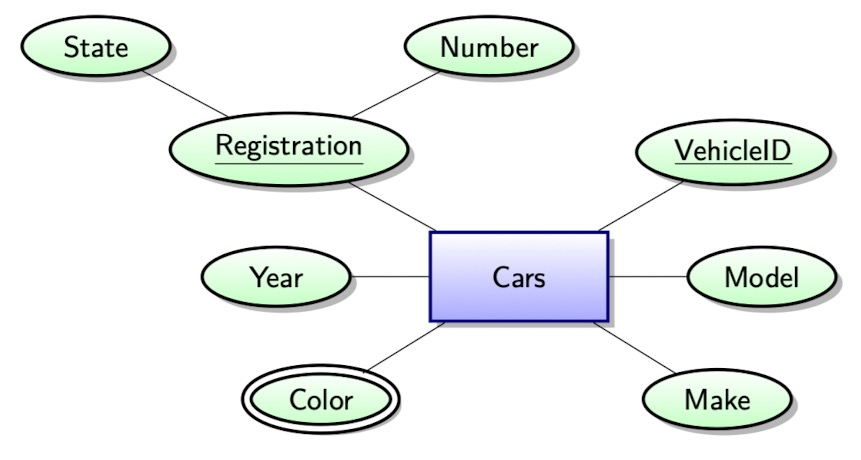
\includegraphics[width=0.5\linewidth]{images/Screenshot 2024-05-22 at 10.13.58.jpg}
    \caption{Entity type Cars}
\end{figure}
\subsubsection{Entity Sets}
The collection of all entities of a particular entity type in the database is called the \textbf{entity set}


\subsection{Relationships, Relationship Types, Relationship Sets}
\begin{itemize}[label=\(\rhd\)]
    \item A \textbf{relationship} relates two or more distinct entities with a specific meaning.
    \begin{itemize}[label=\(\rhd\)]
        \item Example: John Smith \textit{works on} project ProductX
    \end{itemize}
    \item Relationships of the same type are grouped into a \textbf{relationship type}
    \begin{itemize}[label=\(\rhd\)]
        \item E.g., the \textit{workOn} relationship type
    \end{itemize}
    \item The \textbf{degree} of a relationship type is the number of participating entity types
    \begin{itemize}[label=\(\rhd\)]
        \item workOn is a \textit{binary} relationship
    \end{itemize}
\end{itemize}

In ER diagrams relationship types are represented with a diamond-shaped box connected tot the participating entity types


\subsubsection{Strucutral Constraints on Relationships}
\begin{itemize}[label=\(\rhd\)]
    \item \textbf{Cardinality constraint} specifies the \textit{maximum} participation
    \begin{itemize}[label=\(\rhd\)]
        \item One-to-one (1:1)
        \item One-to-many (1:N) or Many-to-one (N:1)
        \item Many-to-Many (N:N)
    \end{itemize}

    \begin{figure}[H]
        \centering
        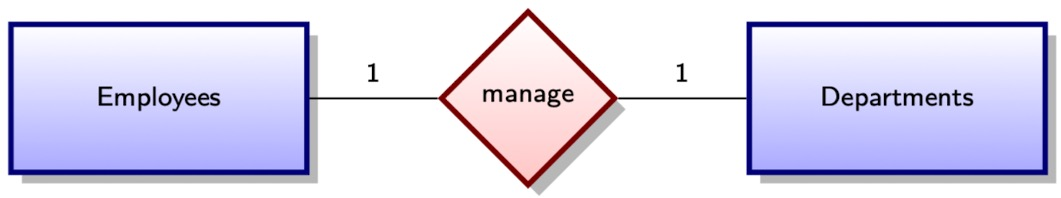
\includegraphics[width=0.5\linewidth]{images/Screenshot 2024-05-22 at 10.33.11.jpg}
        \caption{Cardinality constraint}
    \end{figure}
    \item A \textbf{participation constraint} specifies \textit{minimum} participation (also called existence dependency)
    \begin{itemize}[label=\(\rhd\)]
        \item zero (optional participation)
        \item one or more (mandatory participation)
    \end{itemize}
    \begin{figure}[H]
        \centering
        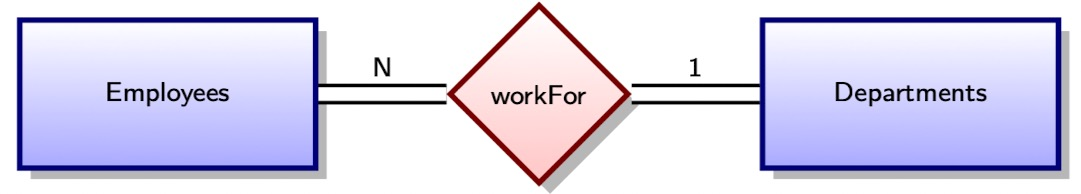
\includegraphics[width=0.5\linewidth]{images/Screenshot 2024-05-22 at 10.33.47.jpg}
        \caption{Participation constraint}
    \end{figure}\begin{itemize}[label=\(\rhd\)]
        \item Means an employee \textit{must} workFor a department
        \item A departement \textit{must} giveWorkTo N employees
    \end{itemize}
\end{itemize}

\subsubsection{Recursive Relationships}

\begin{itemize}[label=\(\rhd\)]
    \item In a \textbf{recursive} relationship type:
    \begin{itemize}[label=\(\rhd\)]
        \item The same entity type participates in different roles (e.g. a employee can be supervisor but also subordinate)
    \end{itemize}
    \item In ER diagrams need to display role names to distinguish participation
\end{itemize}
\subsubsection{Attributes of Relationships}
\begin{itemize}[label=\(\rhd\)]
    \item A relationship type can have attributes: 
    \begin{itemize}[label=\(\rhd\)]
        \item Example: \textit{HoursPerWeek} for the \textit{workOn} relation
    \end{itemize}
\end{itemize}


\subsection{Weak Entities, N-ary Relationships}
\subsubsection{Weak Entities}
\begin{itemize}[label=\(\rhd\)]
    \item A \textbf{weak entity type} is an entity that does not have a key attribute
    \item It must participate in an \textbf{identifying relationship type} with an owner or identifying entity type
    \item Entities are identified by the combination of:
    \begin{itemize}[label=\(\rhd\)]
        \item A partial key of the weak entity type
        \item The particular entity they are related to in the identifying entity type
    \end{itemize}
\end{itemize}
In ER diagrams displayed with two diamond-shapes and weak entity type with two rectangles.

\subsubsection{N-ary Relationships}

\begin{figure}[H]
    \centering
    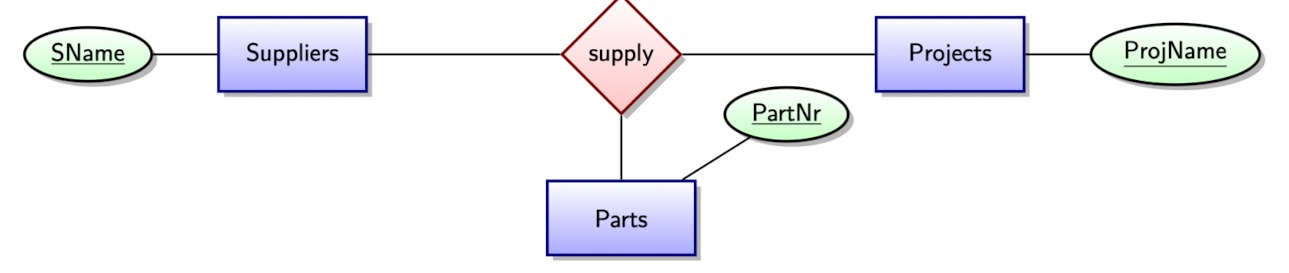
\includegraphics[width=0.5\linewidth]{images/Screenshot 2024-05-22 at 10.42.34.jpg}
    \caption{Ternary Relationship}
\end{figure}

\textbf{\underline{Example:}}
\begin{figure}[H]
    \centering
    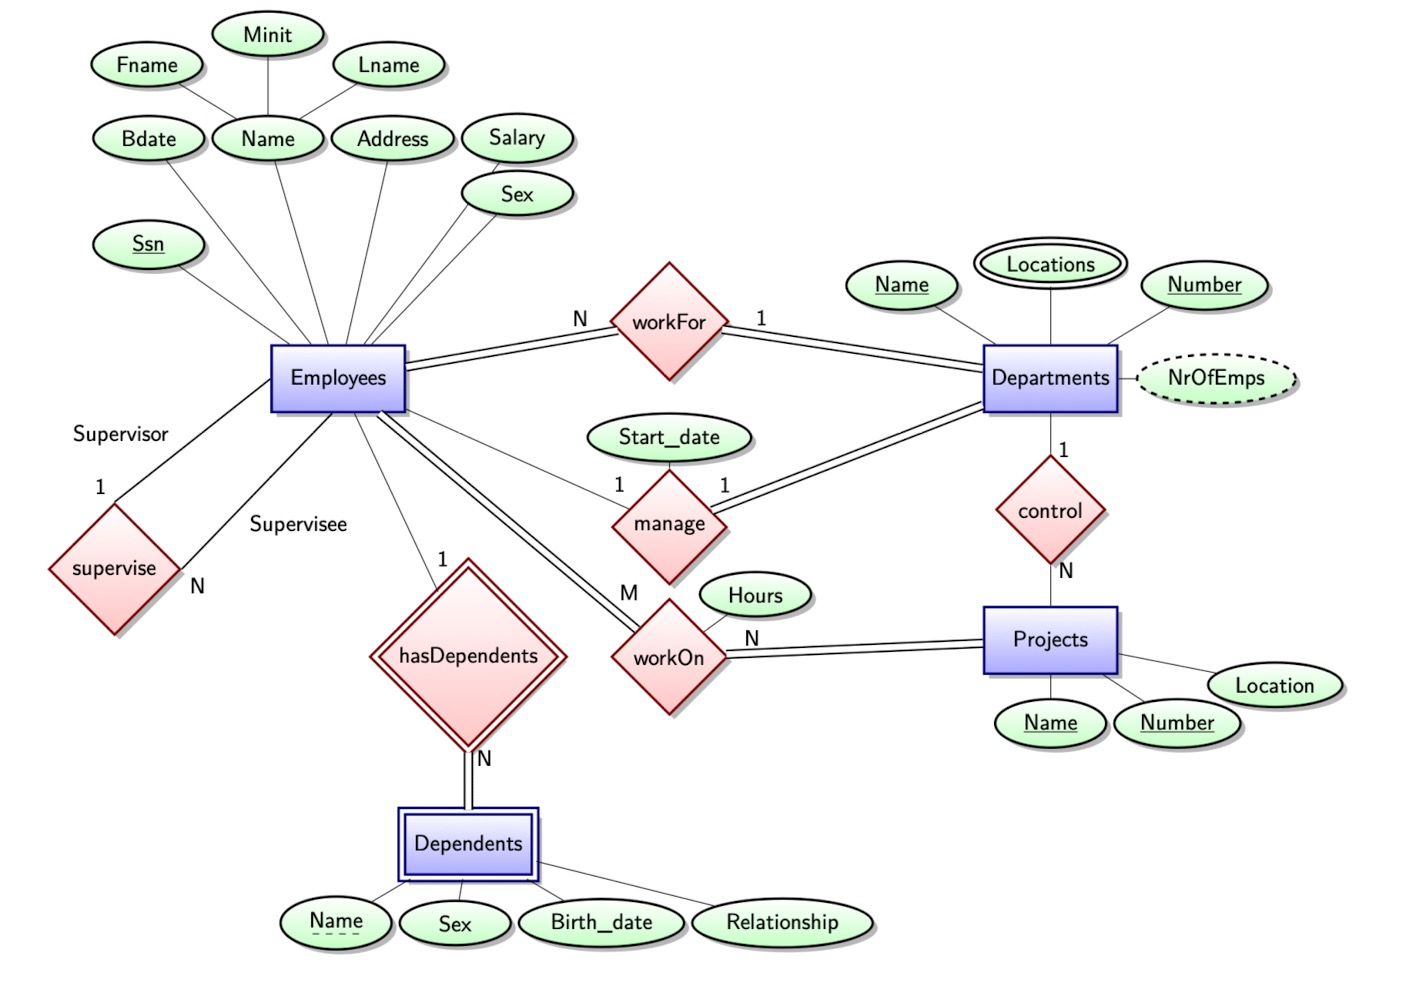
\includegraphics[width=0.75\linewidth]{images/Screenshot 2024-05-22 at 10.45.08.jpg}
\end{figure}

\subsubsection{Summary of ER Diagram Notation}

\begin{figure}[H]
    \centering
    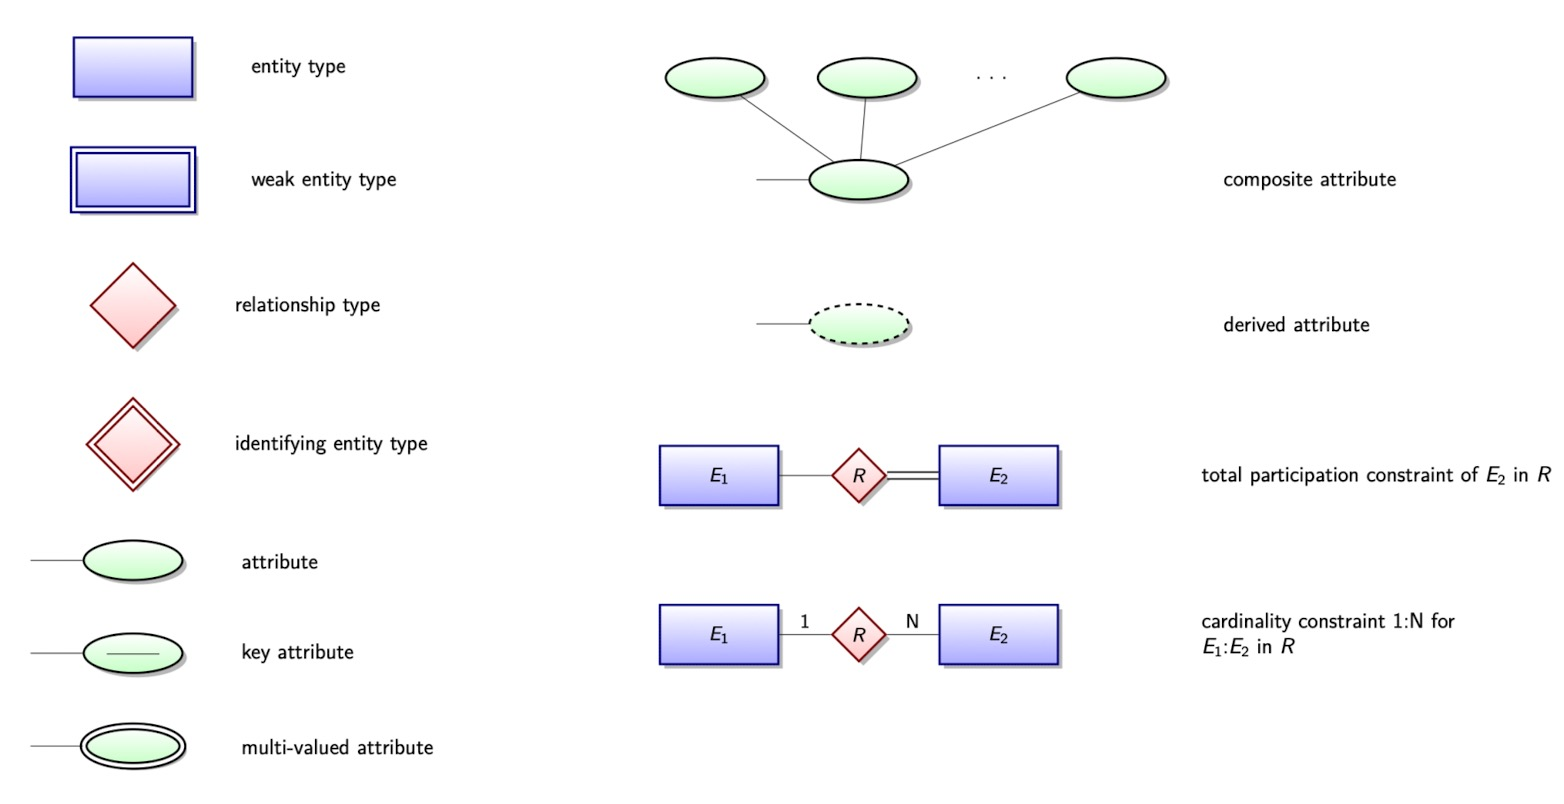
\includegraphics[width=0.75\linewidth]{images/Screenshot 2024-05-22 at 10.46.08.jpg}
\end{figure}


\subsection{Subclasses and Superclasses}
\begin{itemize}[label=\(\rhd\)]
    \item An entity set may have additional meaningful \textbf{subgroupings} that must be represented explicitly because of their significance to applications
    \item ER diagrams represent these subgroupings as \textbf{subtypes} (or \textbf{subclasses})
    \item Superclass/subclass relations are called \textbf{IS-A} relationships
    \item \textbf{Specialization} is the process of defining subclasses of a superclass
    \item \textbf{Generalization} is the reverse of the specialization process
    \item An entity that is member of a subclass \textbf{inherits} all attributes and all relationships of the superclass
\end{itemize}

\begin{figure}[H]
    \centering
    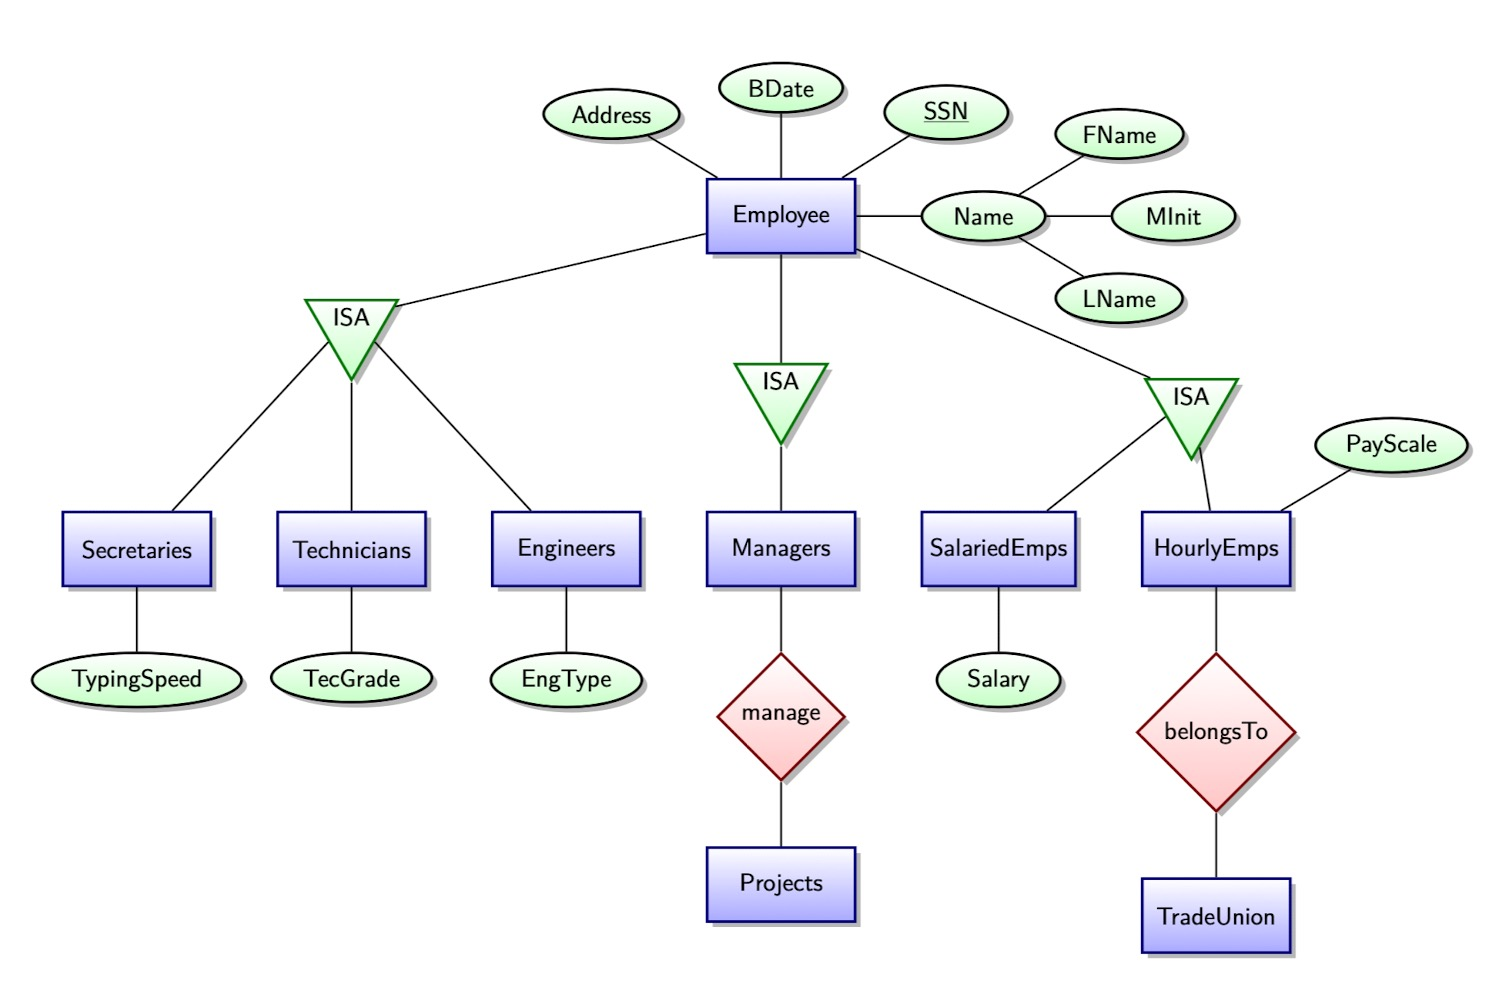
\includegraphics[width=0.75\linewidth]{images/Screenshot 2024-05-22 at 10.51.13.jpg}
\end{figure}

\subsubsection{Disjointness Constraint}
\textbf{Disjointness Constraint}
\begin{itemize}[label=\(\rhd\)]
    \item Specifies that the subclass of the specialization must be \textit{disjoint}
    \begin{itemize}[label=\(\rhd\)]
        \item An entity can be a member of at most one of the subclasses of the specialization 
        \item If not disjoint, specialization is \textit{overlapping}
    \end{itemize}
    \item In ER diag. shown by a anotation \textit{disjoint} next to line
\end{itemize}
\subsubsection{Completeness Constraint}
\textbf{Completeness Constraint}
\begin{itemize}[label=\(\rhd\)]
    \item \textit{Total} specifies that every entity in the superclass must be a member of some subclass in the specialization/generalization 
    \item In ER diag. shown by double line
\end{itemize}

Hence, there are four types of specialization/generalization:
\begin{itemize}[label=\(\rhd\)]
    \item Disjoint, total
    \item Disjoint, partial
    \item Overlapping, total
    \item Overlapping, partial
\end{itemize}


\subsection{ER-to-Relational Mapping Algorithm}


\subsubsection{Mapping an ER Model to a Relational Model}
\begin{itemize}[label=\(\rhd\)]
    \item \textbf{Step 1: Mapping of Regular Entity Types}
    \begin{itemize}[label=\(\rhd\)]
        \item For each regular (strong) entity type E in the ER schema, create a relation schema $R$ that includes all the simple attributes of E
        \item A composite is flattened into a set of simple attributes
        \item Choose one of the key attributes of E as the primary key for $R$
    \end{itemize}
    \item \textbf{Step 2: Mapping of Weak Entity Types}
    \begin{itemize}[label=\(\rhd\)]
        \item For each weak entity type W in the ER diagram with owner entity type E, create a relation schema $R$ and include all simple attributes (or simple components of composite attributes) of W as attributes
        \item Include as foreign key attributes of $R$ the primary key attributes of the relations that correspond to the owner entity types
        \item The primary key of $R$ is the \textit{combination} of the primary keys of the owners and the partial key of the weak entity type W, if any.
    \end{itemize}
    \item \textbf{Step 3: Mapping of Binary 1:1 Relation Types}
    \begin{itemize}[label=\(\rhd\)]
        \item For each binary 1:1 relationship type r in the ER schema, identify the relation schemas $S$ and $T$ that correspond to the entity types participating in r
        \item There are three possible approaches:
        \begin{enumerate}
            \item \textbf{Foreign Key Approach:} Choose one of the relations and include as foreign key the primary key of the other relation (Better to choose an entity type with total participation)
            \item \textbf{Merged  Relation Option:} An alternate mapping of 1:1 relationship type is possible by merging the two entity types and the relationship into a single relation (May be appropriate if both participations are total)
            \item \textbf{Cross-reference or relationship relation option:} The third alternative is to set up a third relation schema $R$ for the purpose of cross-referencing the primary keys of the two relation schemas $S$ and $T$ representing the entity types
        \end{enumerate}
    \end{itemize}
    \item \textbf{Step 4: Mapping of Binary 1:N Relationship Types}
    \begin{itemize}[label=\(\rhd\)]
        \item For each binary 1:N relationship type r, identify the relation schemas $S$ and $T$ that correspond to the entity types participating in r. $S$ is the N-side
        \item Include as foreign key in $S$ the primary key of $T$ that represents the other entity type participating in r
        \item Include simple attributes of the 1:N relation types as attributes of $S$
    \end{itemize}
    \item \textbf{Step 5: Mapping of Binary M:N Relationship Types}
    \begin{itemize}[label=\(\rhd\)]
        \item For each regular M:N relationship type r, \textit{create a new relation schema} $S$ to represent r
        \item Include as FK attributes in $S$ the PK of the relations that represent the participating entity types: \textit{their combination will form the primary key of} $S$
        \item Also include any simpe attributes of the M:N relationship type as attributes of $S$
    \end{itemize}
    \item \textbf{Step 6: Mapping of Multivalued Attributes}
    \begin{itemize}[label=\(\rhd\)]
        \item For each multivalued attribute A, create a new relation schema $R$
        \item $R$ includes an attribute A, plus the PK attribute $K$ of the relation that represents the entity or relationship type that has $A$ as an attribute
        \item The primary key of $R$ is the combination of $A$ and $K$
    \end{itemize}
    \item \textbf{Step 7: Mapping of N-ary Relationship Types}
    \begin{itemize}[label=\(\rhd\)]
        \item For each n-ary relationship type r, where n>2, create a relation schema $S$
        \item Include as FK attributes in $S$ the PKs of the relations that represent the participating entity types
        \item Also include any simple attributes of the n-ary relationship type
    \end{itemize}
    \item \textbf{Step 8: Options for Mapping Specialization or Generalization}
    \begin{itemize}[label=\(\rhd\)]
        \item Convert each specialization with $m$ subclasses $S_1,S_2,...,S_m$ and superclass C, where the attributes of C are $k,a_1,...,a_n$ and $k$ is the PK, into relation schemas using one of the four following options:
        \begin{itemize}[label=\(\rhd\)]
            \item \textbf{Option 8A: Multiple relations for superclass and subclasses}
            \begin{itemize}[label=\(\rhd\)]
                \item Create a relation schemas $L$ for C with attributes \[Attrs(L)=\{k,a_1,...,a_n\} \text{ and } PK(L)=k\]
                \item Create a relation schema $L_i$ for each subclass $S_i$, $1<i<m$, with attributes $Attrs(L_i)=\{k\} \cup \{attributes\ of\ S_i\}$ and $PK(L_i)=k$
                \item This option works for any specialization
            \end{itemize}
            \item \textbf{Option 8B: Multiple relations for subclass relations only}
            \begin{itemize}[label=\(\rhd\)]
                \item Create a relation $L_i$ for each subclass $S_i$, $1<i<m$, with attributes\\ $Attr(L_i)\{attributes\ of\ S_i\} \cup \{k,a_1,...,a_n\}$ and $PK(L_i)=k$
                \item This option only works for a specialization whose subclasses are total
            \end{itemize}
            \item \textbf{Option 8C: Single relation with one type attribute}
            \begin{itemize}[label=\(\rhd\)]
                \item Create a single relation $L$ with attributes $Attr(L)=\{k,a_1,...a_n\} \cup \{attributes\ of\ S_1\} \cup \{attributes\ of\ S_m\}$ and $PK(L)=k$
                \item The attribute $t$ is called a type attribute that indicates the subclass to which each tuple belongs
                \item This option only works for specialization whose subsclasses are disjoint and might generate many null values for attributes of subclasses
            \end{itemize}
            \item \textbf{Option 8D: Single relation with multiple type attributes}
            \begin{itemize}[label=\(\rhd\)]
                \item Create a single relation $L$ with attributes \\ $Attr(L) = \{k,a_1,...a_n, t_1,...,t_m\} \cup \{attributes\ of\ S_1\} \cup \{attributes\ of\ S_m\}$ and $PK(L)=k$ 
                \item Each $t_i$ is a Boolean attribute that indicates whether a tuple belongs to subclass $S_i$
                \item This option works for a specialization whose subclasses are overlapping (but will also work for disjoint)
            \end{itemize}
        \end{itemize}
    \end{itemize}
\end{itemize}

\subsection{Summary}
Correspondence between ER and Relational Models


\begin{table}[H]
    \centering
    \begin{tabular}{|c|c|}
    \hline
         \textbf{ER Model} & \textbf{Relational Model} \\
         \hline 
         Entity type & Entity relation \\
                  \hline 
         1:1 or 1:N relationship type & Foreign key (or relationship relation) \\
                  \hline 
         M:N relationship type & Relationship relation and two foreign keys \\
                  \hline 
         n-ary relationship type & Relationship relation and n foreign keys \\
                  \hline 
         Simple attribute & Attribute \\
                  \hline 
         Composite attribute & Set of simple component attributes \\
                  \hline 
         Multivalued attribute & Relation and foreign key \\
                  \hline 
         Key attribute & Primary (or secondary) key \\
                  \hline 
    \end{tabular}
\end{table}